% Chapter 4: System Architecture and Design
\chapter{System Architecture and Implementation}
\label{chap:architecture}

\setlength{\parskip}{1em}

This chapter details the architecture and implementation of the core security toolkit. The system is designed as a modular and extensible command-line interface (CLI) application, enabling developers to easily integrate security scanning into their workflow.

\section{System Architecture}

The toolkit is architected in Python, chosen for its extensive standard library, rich third-party package ecosystem, and suitability for scripting and automation. The high-level architecture is centered around a core orchestrator and a set of pluggable scanner modules.

\begin{itemize}
    \item \textbf{Core Orchestrator (\texttt{main.py}):} This is the central component of the application. It is responsible for parsing user commands and options, loading the appropriate scanner modules, and managing the flow of data from the scanners to the output handlers. It is built using the \texttt{Typer} library to provide a clean and modern command-line interface.
    \item \textbf{Scanner Modules:} Each security scanner is implemented as a separate Python module (e.g., \texttt{injection.py}, \texttt{cryptographic\_failures.py}). This modular design allows for clear separation of concerns and makes the system easy to extend. Each module is responsible for a specific type of vulnerability detection, following the categories outlined in the OWASP Top 10.
    \item \textbf{Input/Output Handlers:} The toolkit is designed to be flexible in its input and output. It can scan individual files or entire directories. The results are presented in two formats: a human-readable summary table for quick assessment and a machine-readable JSON file for integration with other tools and CI/CD pipelines. The \texttt{rich} library is used to enhance the presentation of output in the terminal.
\end{itemize}

\begin{figure}[h!]
\centering
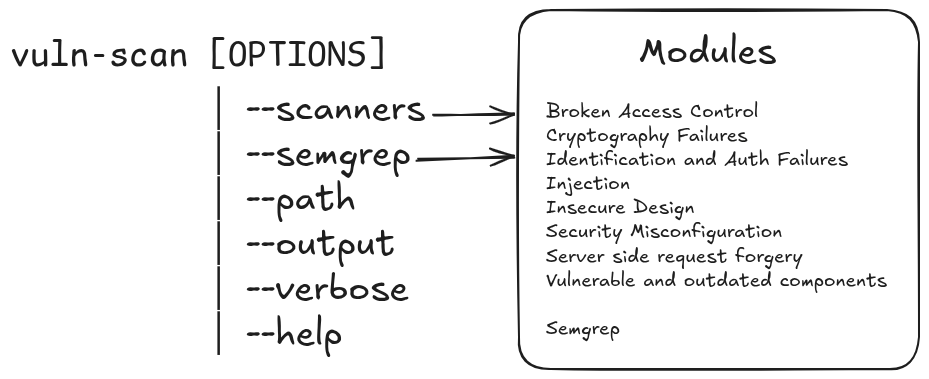
\includegraphics[width=0.75\textwidth]{images/CLI-Diagram.png}
\caption{High-level system architecture showing the CLI interface, Core Orchestrator, two scanning engines (Custom Engine and Semgrep Engine), and the associated scanner modules.}
\label{fig:system_architecture}
\end{figure}

The overall workflow is as follows:
\begin{enumerate}
    \item The user invokes the tool via the command line, specifying which scanners to run and the target path.
    \item The core orchestrator parses these arguments.
    \item It dynamically loads and executes the selected scanner modules on the target files.
    \item Each scanner returns a list of identified issues.
    \item The orchestrator aggregates the results from all scanners.
    \item The results are then formatted and presented to the user, either as a table in the console or as a JSON file.
\end{enumerate}

\section{Choice of Programming Language}

During the initial planning phase of this project, the Rust programming language was considered as a potential candidate for implementation. Rust is known for its performance, memory safety, and strong type system, which are all desirable qualities for a security-focused tool. However, during the research and implementation phase, it became apparent that the steep learning curve of Rust, combined with the strict project deadlines, would pose a significant risk to the timely completion of the project.

Given these constraints, a pragmatic decision was made to switch to Python. Python was chosen for its extensive standard library, rich ecosystem of third-party packages (such as \texttt{Typer} and \texttt{rich}), and its overall ease of development. This allowed for a more rapid development cycle and enabled a stronger focus on the core logic and features of the security toolkit, rather than on the intricacies of a new programming language. This trade-off allowed for the successful implementation of the project within the given timeframe.

\section{Implementation Details}

The main entry point of the application is \texttt{main.py}. This script is responsible for parsing command-line arguments, orchestrating the execution of selected security scanners, and presenting the results to the user.

The core of the CLI is the \texttt{scan} command, which is defined using a \texttt{Typer} decorator. This command serves as the primary interface for the user to interact with the toolkit.

\begin{minted}{python}
@app.command()
def scan(
    scanners: str = typer.Option(
        ...,
        "--scanners",
        "-s",
        help="Comma-separated list of scanners to run (e.g. bac,crypto) or 'all'.",
    ),
    path: Path = typer.Option(
        Path("."), "--path", "-p", help="File or directory to scan (defaults to current dir)."
    ),
    output: str = typer.Option(None, "--output", "-o", help="Optional JSON output file."),
    verbose: bool = typer.Option(
        False,
        "--verbose",
        "-v",
        help="Enable verbose output, showing detailed information about the scan.",
    ),
):
    """Run one or more vulnerability scanners."""
    # ...
\end{minted}

The \texttt{scan} command is designed around two primary, mutually exclusive scanning modes:
\begin{itemize}
    \item \textbf{--scanners (-s):} Activates the \textbf{Custom Engine}. The user can provide a comma-separated list of scanner names (e.g., `bac,crypto`) or specify `all` to run every custom module.
    \item \textbf{--semgrep:} Activates the \textbf{Semgrep Engine}, running Semgrep on the target path. This provides an alternative scanning strategy focused on broad, pattern-based analysis.
\end{itemize}

This design gives the user direct control over the scanning methodology. The core logic ensures that only one engine can be run at a time to prevent conflicting or redundant results.

\subsection{Engine Orchestration}

The toolkit's core logic, located in `main.py`, parses the user's choice of engine.

If the `scanners` flag is used, the application iterates through the `SCANNERS` dictionary, which maps custom scanner names to their respective functions, and executes them.

If the `--semgrep` flag is chosen, the tool instead calls the `scan\_semgrep` function. This module acts as a wrapper, executing Semgrep as a subprocess and formatting its JSON output to align with the toolkit's reporting structure. This integration makes Semgrep a first-class component of the tool, not just an external utility.


\begin{minted}{python}
SCANNERS = {
    "broken_access_control": scan_bac,
    "cryptographic_failures": scan_crypto,
    "injection": scan_injection,
    "insecure_design": scan_insecure_design,
    "security_misconfiguration": scan_sm,
    "vulnerable_and_outdated_components": scan_vaoc,
}
\end{minted}

The application normalizes the user's input for the \texttt{--scanners} option, allowing for aliases and handling the \texttt{all} keyword. This logic ensures flexibility and ease of use.

\begin{minted}{python}
if scanners.lower() == "all":
    selected_scanners = list(SCANNERS.keys())
else:
    selected_scanners = []
    for name in scanners.split(","):
        name = name.strip()
        if name in ALIASES:
            name = ALIASES[name]
        if name not in SCANNERS:
            typer.secho(f"Error: Scanner '{name}' not found.", fg=typer.colors.RED)
            raise typer.Exit(1)
        selected_scanners.append(name)
\end{minted}

The application then iterates through the selected scanners, determines the target files for each, and executes the scan. A special case is handled for the \texttt{vulnerable\_and\_outdated\_components} scanner, which specifically looks for dependency management files like \texttt{requirements.txt}, \texttt{pyproject.toml}, \texttt{poetry.lock}, or \texttt{Pipfile.lock}. Other scanners recursively search for Python (\texttt{*.py}) files within the target directory.

\section{Scanner Module Details}
\label{sec:scanner_modules}

Each scanner is tailored to a specific OWASP Top 10 category, employing different techniques to identify potential vulnerabilities. 

\subsection{Broken Access Control}
This module targets vulnerabilities related to improper access control enforcement. It statically analyzes Python source code using the \texttt{ast} library to parse the code into an Abstract Syntax Tree. The scanner walks through the tree to identify several patterns:
\begin{itemize}
    \item \textbf{Hardcoded Roles:} Assignment of privileged roles (e.g., \texttt{"admin"}, \texttt{"superuser"}) as string literals.
    \item \textbf{Insecure Direct Object References (IDOR):} Direct use of user-controllable input from web request objects (e.g., \texttt{request.args.get()}) in security-sensitive contexts, such as database queries, which could allow users to access unauthorized data.
    \item \textbf{Insecure Route Parameters:} Use of common identifiers like \texttt{userid} or \texttt{username} as parameters in Flask routes, which may indicate a potential IDOR vulnerability.
\end{itemize}

\subsection{Cryptographic Failures}
This module focuses on identifying weaknesses in the use of cryptography. It also uses \texttt{ast} parsing to detect the the following issues:
\begin{itemize}
    \item \textbf{Weak Hashing Algorithms:} Use of outdated and insecure hashing functions such as \texttt{MD5} and \texttt{SHA1}.
    \item \textbf{Weak Cipher Algorithms and Modes:} Use of deprecated ciphers like \texttt{DES} or insecure block cipher modes like Electronic Codebook (\texttt{ECB}).
    \item \textbf{Insecure Randomness:} Use of the standard \texttt{random} module for security-sensitive operations, which is not cryptographically secure. The \texttt{secrets} module should be used instead.
    \item \textbf{Hardcoded Secrets:} Detection of hardcoded passwords, API keys, and JWT secrets, which should be loaded from a secure configuration source.
\end{itemize}

\subsection{Injection}
The injection module scans for vulnerabilities where untrusted data can be sent to an interpreter as part of a command or query. It uses a hybrid approach of \texttt{ast} parsing and regular expression matching.
\begin{itemize}
    \item \textbf{Command Injection:} Detects the use of functions like \texttt{os.system} and \texttt{os.popen} that execute system commands.
    \item \textbf{Code Injection:} Flags the use of dangerous built-in functions like \texttt{eval()} and \texttt{exec()}.
    \item \textbf{SQL Injection:} Identifies the use of raw SQL queries, particularly with unsafe string formatting (e.g., f-strings or \texttt{\%}-formatting) in database cursor \texttt{execute()} methods.
\end{itemize}

\subsection{Insecure Design}
This module is designed to catch broad, architecture-level weaknesses. In its current implementation, it focuses on a particularly dangerous design choice: the use of \texttt{eval()}. The scanner uses \texttt{ast} parsing to find any calls to this function, as it can execute arbitrary code and often represents a significant security risk.

\subsection{Security Misconfiguration}
This module searches for common misconfigurations in application setups. Unlike other modules, it performs a direct text search on files rather than parsing the code structure. Its primary target is identifying when a Flask web application is running in debug mode (\texttt{app.run(debug=True)}) in a production environment, which can expose sensitive information and allow for arbitrary code execution.

\subsection{Vulnerable and Outdated Components}
This scanner addresses the risk of using software components with known vulnerabilities. It operates differently from the static analysis modules by integrating with the \texttt{pip-audit} tool. It scans dependency management files such as \texttt{requirements.txt}, \texttt{pyproject.toml}, \texttt{poetry.lock}, and \texttt{Pipfile.lock}. The module executes \texttt{pip-audit}, parses its JSON output, and reports any identified vulnerable dependencies.

\subsection{Results Presentation}


To provide a clear and actionable summary of the scan results, the toolkit uses the \texttt{rich} library. A summary table is generated to show the number of issues found by each scanner.

\begin{minted}{python}
table = Table(title="All Scanners Summary")
table.add_column("Scanner", style="cyan", no_wrap=True)
table.add_column("Issues Found", justify="right", style="magenta")

for scanner_name in selected_scanners:
    issues = results_by_scanner[scanner_name]
    table.add_row(scanner_name.replace("_", " ").title(), str(len(issues)))

console.print(table)
\end{minted}

Finally, the detailed results are provided in JSON format. This can be either written to a file specified by the \texttt{--output} option or printed directly to the console using \texttt{rich}'s JSON printing capabilities, which includes syntax highlighting for better readability. This dual-output functionality supports both interactive use and integration into automated CI/CD pipelines.

\begin{minted}{python}
if output:
    with open(output, "w", encoding="utf-8") as f:
        json.dump(results_by_scanner, f, indent=4)
    typer.secho(f"Results saved to {output}", fg=typer.colors.GREEN)
else:
    print_json(data=results_by_scanner)
\end{minted}